\section{Method}

\todo[inline]{Explain why measurements, and how measurements.}

\subsection{How measurements will be performed}

\subsection{The creation of a RBN}

\subsection{The creation of a functioning RRC system}

The training process for a RRC system is threefold.

First, we create a number of datasets for training,
as well as a dataset for later testing.
These datasets are either Temporal Parity or Density,
as described in section \ref{subsection:rbn-reservoir-systems}.

We then either create a new RBN (initialize it randomly),
or load a previously created RBN from disk.

For each bit of input in each dataset,
we perturb the input-connected nodes in the RBN.
After each perturbance, the RBN is ran synchronously (CRBN mode) for one timestep.
The resulting RBN states are collected,
and after the entire dataset is processed,
forwarded to the readout layer.

To find a suitable mapping from the set of reservoir states and the correct input classification,
ridge regression \cite{hoerl1970ridge} is used.
This version of least squares regression is more accurate when faced with input colinearities,
as well as always being at least as accurate as ordinary least squares.

This process is repeated for all the datasets,
and the final regression parameters are chosen as a combination of the parameters obtained for each individual dataset.
Finally we measure the normalized accuracy of the trained reservoir on the test dataset,
defined as
\begin{equation}
Accuracy = 1 - \dfrac{sum(actual\_output \neq expected\_output)}{len(correct\_output)}
\label{formula:accuracy}
\end{equation}
.
If the RRC system achieved a high accuracy on an interesting task,
it can be stored ('pickled') to disk for further research.

\subsection{The evolving of functionally similar RBNs for existing readout layers}

To investigate the potential many-to-one mapping between RBN-reservoirs and readout layers,
we'll be using a genetic algorithm to evolve candidate RBNs,
using a fixed test dataset and readout layer for fitness evaluation.

A genetic algorithm is an advanced probabilistic search method using operations inspired by natural evolution to traverse the solution space of the problem.
It mimics natural evolution by creating a population of children where some will grow up to adults,
the fittest of which reproduce the most.
The newly created offspring receives a genome derived from its parents,
using a combination of genome crossover and random mutations to push the search forward.

Good choices for genome representations and fitness functions make GAs excellent for finding solutions to optimisation problems.
Good hyperparameters (parameters for the GA run itself, i.e. crossover rate, adult and child population sizes)
have to be found for each separate problem domain due to the No Free Lunch Theorem.

\subsubsection{Genotype and phenotype representation}

We let the genotype be a direct encoding of the corresponding RBN graph.
Such an encoding is significantly larger than a generative encoding,
but less complex as well as able to generate all individuals in the fitness landscape.

Each node needs to represent whether it is connected to the input node,
who its neighbors are, and what its transition rule is.
As we only look at homogenous RBNs,
we can use a fixed-length genome with
\begin{equation}
genome\_length = n\_nodes \cdot (connectivity + 2)
\end{equation}
To further simplify GA implementation,
we let all symbols in the genome take a value in the range $[0, max\_required\_in\_genome)$.
The actual symbol values are then computed modulo the largest actual value they could take on
(2 for input connectivity, n\_nodes for neighbors, $2^{2^{n\_nodes}}$ for transition rules).
This redundancy in the genome can be an advantage,
as it allows for new ways to explore the fitness landscape \cm.

The final genome is shown in figure \ref{figure:rbn-genotype}.
Note that this representation sets no limitations on input connectivity or uniqueness of neighbors.

\begin{figure}
  \centering
  \begin{bytefield}[bitwidth=1.5em]{12}
    \bitheader{0-11} \\
    \bitbox{1}{C} \bitbox{1}{N\textsubscript{1}} \bitbox{1}{N\textsubscript{2}} \bitbox{1}{R}
    \bitbox{1}{C} \bitbox{1}{N\textsubscript{1}} \bitbox{1}{N\textsubscript{2}} \bitbox{1}{R}
    \bitbox{1}{C} \bitbox{1}{N\textsubscript{1}} \bitbox{1}{N\textsubscript{2}} \bitbox{1}{R} \\
    \bitbox[t]{4}{$\underbrace{\hspace{6em}}_{\text{\normalsize Node 1}}$}
    \bitbox[t]{4}{$\underbrace{\hspace{6em}}_{\text{\normalsize Node 2}}$}
    \bitbox[t]{4}{$\underbrace{\hspace{6em}}_{\text{\normalsize Node 3}}$} \\
  \end{bytefield}
  \caption{
    The direct-encoded genotype used for evolving RBNs,
    shown here for an RBN with $N=3, K=2$.}
  \label{figure:rbn-genotype}
\end{figure}

\subsubsection{Fitness function}

Each GA run is parameterized with an already-trained and accurate readout layer (separated from its RBN-reservoir),
as well as a single test dataset of the same origins as the dataset used for training the readout layer.
After converting each genotype to its corresponding phenotype,
the resulting RBN is connected to the readout-layer and fed with the fixed test dataset.
The accuracy obtained,
as calculated in formula \ref{formula:accuracy},
is used as the fitness of the phenotype.

\subsubsection{GA hyperparameters}

The hyperparameters for the GA are presented in table \ref{table:ga-hyperparameters}.

\begin{table}
  \centering
  \caption{GA hyperparameters}
  \label{table:ga-hyperparameters}
  \begin{tabular}{ll}
    Children pool size             & 40                                    \\
    Adult pool size                & 40                                    \\
    Fitness satisfaction threshold & 0.98                                  \\
    maximum generations            & 200                                   \\
    Adult selection                & Generational mixing                   \\
    Parent selection               & Tournament selection(K=8)             \\
    Genome crossover               & Per component crossover (p=0.5)       \\
    Genome mutation                & Per genome component mutation (p=0.1) \\
  \end{tabular}
\end{table}

Adult selection is simple generational mixing,
selecting the best 40 specimens from the combined children and adult populations.
Per component crossover will with a probability p either pass through the entire genome from the left parent,
or for each component chose either the left or right parents value with a probability 0.5.
Per genome component mutation will reroll each genome component with probability p.
This value is set relatively high (0.1) due to experiments showing a much faster convergence rate than with the initial chosen value of 0.01.

The temporal parity task will be used for evaluating the evolved RBNs with parameters as set in table \ref{table:dataset-parameters}.

\begin{table}
  \centering
  \caption{Task parameters}
  \label{table:dataset-parameters}
  \begin{tabular}{ll}
    Task type       & Temporal Parity \\
    Dataset length  & 200             \\
    Window size (N) & 3               \\
    Offset (T)      & 0               \\
  \end{tabular}
\end{table}

\subsection{Find some other place for this?}

It seems that for a random sample of reservoirs of a given size and connetivity,
the temporal density task is solveable for a larger $ n $ than the temporal parity one.
The parity task might therefore requires a more specialized network topology to function well.
Due to the seemingly increased complexity of separating the temporal parity task at low $ n $,
it was chosen as the main task in this paper.

\todo[inline]{Talk a bit about required reservoir complexity, as measured in that previous papaer here?}
\subsection{Measuring dynamics}

\begin{itemize}
  \item
    How do i estimate computational power?
    Use the complexity measure from \cite{rbn-reservoir} of course!
  \item
    How do i estimate transient times and attractor lengths?
    Random samling! Link to some algorithm i use here
  \item
    Fun Anecdote: Link to that paper measuring power usage in RBN-Reservoirs:
    \cite{rbn-reservoir-energy-efficiency}
\end{itemize}

Attractor lengths and such: This might be useful \cite{berdahl2009random}


\subsection{Weaknesses}

\begin{itemize}
  \item Extremely large state-space
  \item Can be difficult to generalize results
  \item
    Genome representation, inefficient, better with binary string?
    Luckily dominated by RBN-Reservoir simulation time
\end{itemize}


\subsection{Experimental setup}

To verify that RBN simulation is working as expected,
a RBN is created randomly, initial state set to all zeros, and ran.
The results are visualized in figure \ref{figure:rbn-noperturb}.
We see that the RBN exhibits stable dynamics, and enters into an attractor around $t=15$.
In figure \ref{figure:rbn-perturb} we continiously perturb the RBN with the input stream from the Temporal Parity task visualized in \ref{figure:temporal-parity}.
In the perturbed case, the state trajectory is continiously changed, preventing the RBN from settling into an attractor.
Interestingly enough, there seems to be a visual similarity between the two cases.
Such a pattern is sure to dissapear with a RBN in the chaotic phase.

This erratic pattern of state transitions is then fed into the readout layer,
which is then tasked with finding a linear combination of the RBN states that results in the expected output for the given task.

\begin{figure}
  \subfloat[Unperturbed]{
    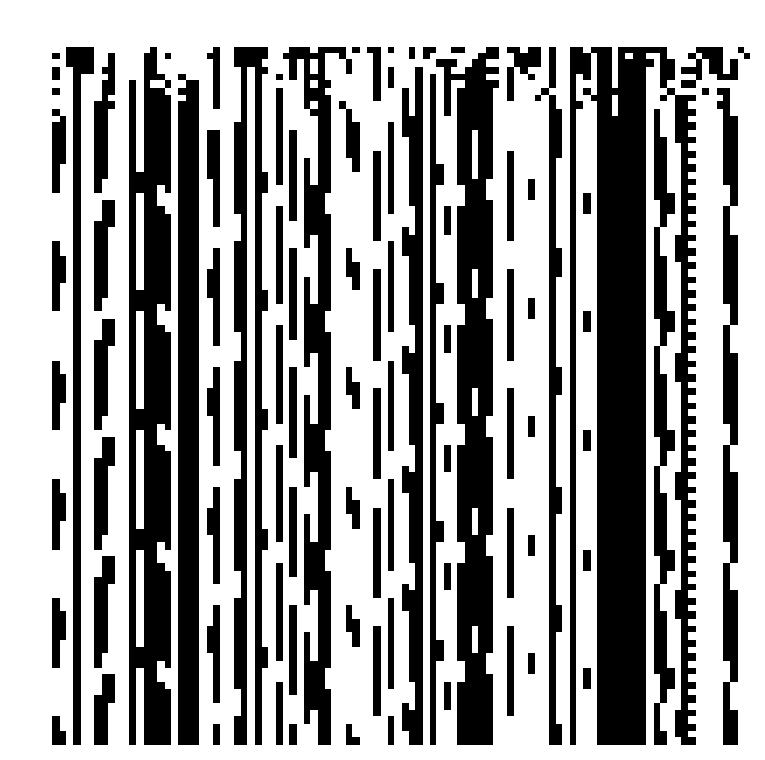
\includegraphics[width=0.5\columnwidth]{method/final-1-noperturb.pdf}
    \label{figure:rbn-noperturb}
  }
  \subfloat[Perturbed]{
    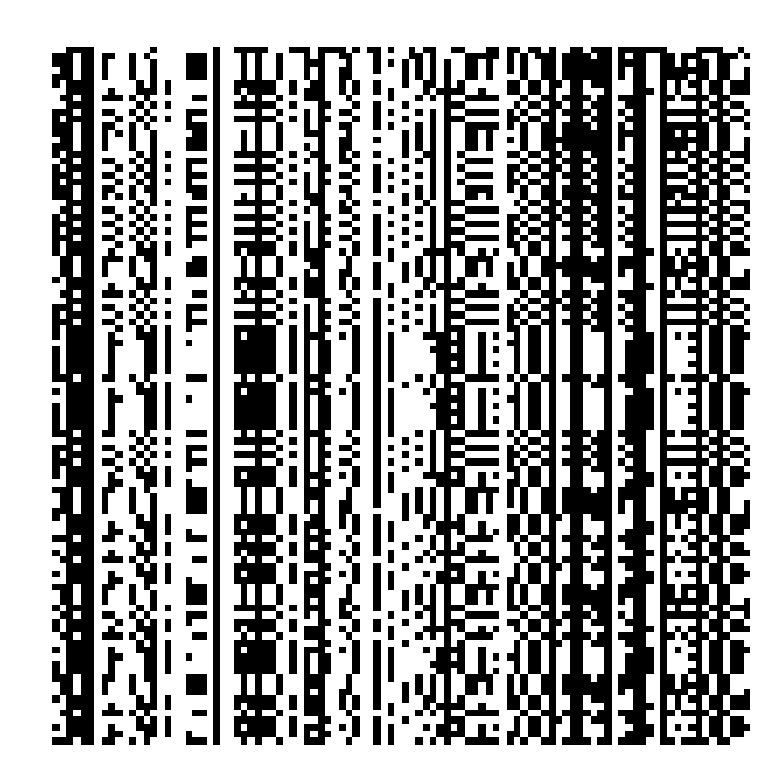
\includegraphics[width=0.5\columnwidth]{method/final-1-perturb.pdf}
    \label{figure:rbn-perturb}
  }
  \caption{
    The same RBN both perturbed and unperturbed.
    Time flows downwards the Y-axis,
    and the current value of each of the nodes in the RBN along the X-axis.
    A cell is white if the value is 1, otherwise black.
    N=100, K=2, P=0.5, L=50, Initial state=0
  }
\end{figure}
